\chapter{Save Page}

The Save Page is used to copy track data from the Machinedrum to a specific slots in the current row of the Grid. \\
\\
When a track is saved to a slot, the MC's internal sequencer data for that track is also stored alongside the copied track data.\\
\\
Master Effects settings are also saved with each MD Track.
\\\\
\textit{The Save Page is accessible from the GridPage by pressing the  \textbf{[Save]} function button.}
\\\\
	\fbox{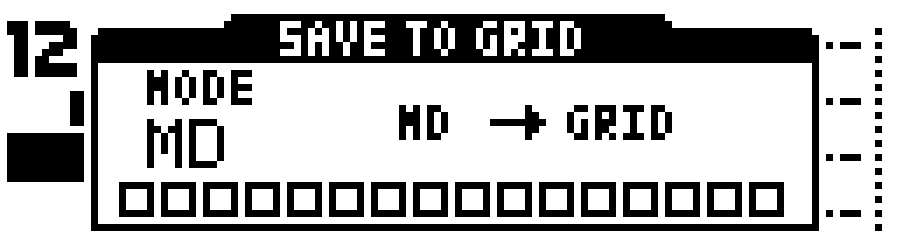
\includegraphics[scale=.40]{save_page.png}}
\section{Encoder Assignment:}
\begin{itemize}
	\item \textbf{[ Encoder 1 ]: }Source Bank
	\item \textbf{[ Encoder 2 ]: }Source Pattern
	\item \textbf{[ Encoder 3 ]: }--
	\item \textbf{[ Encoder 4 ]: }--
\end{itemize}
\section{Saving Tracks}
The Save Page uses the Trigger Interface to specify which tracks are to be saved. Pressing multiple triggers on the MD and then releasing them will cause the selected tracks to be stored in the corresponding slots of the current row.\\
\\
The default behaviour is to store tracks to slots in a one-to-one mapping. That is to stay. Pressing triggers 1,2,3,4 will store MD tracks 1,2,3,4 in MC slots 1,2,3,4 of the current row.\\
\\
Holding  \textbf{[Shift1]} will cause the mapping to be offset by the MD's current track number. For example: If the MD currently has track 5 selected and triggers 1,2,3,4 are chosen then the MD Track's 5,6,7,8 will be stored in slots 1,2,3,4 of the current row.
\section{Store a pattern/row:}
To save an entire pattern/row press \textbf{[Shift2]} from within the Save Page.
All A4 sounds or external sequencer data will also be saved.



\section{Pattern Selection:}

Changing the Bank+Pattern allow you to specify the MD's source pattern location. The MD’s currently loaded pattern and kit are used by default
